\section{Basic Skeletons}

With the \code{ArrowParallel} typeclass in place and implemented, we can now implement some basic parallel skeletons.

\subsection{parEvalNLazy}
\begin{center}
	\includegraphics[scale=0.7]{images/parEvalNLazy}
\end{center}
\code{parEvalN} is 100\% strict, which means that it fully evaluates all passed arrows. Sometimes this might not be feasible, as it will not work on infinite lists of functions like e.g. \code{map (arr . (+)) [1..]} or just because we need the arrows evaluated in chunks. \code{parEvalNLazy} fixes this. It works by first chunking the input from \code{[a]} to \code{[[a]]} with the given \code{ChunkSize} in \code{(arr \$ chunksOf chunkSize)}. These chunks are then fed into a list \code{[arr [a] [b]]} of parallel arrows created by feeding chunks of the passed \code{ChunkSize} into the regular parEvalN by using \code{listApp}. The resulting \code{[[b]]} is lastly converted into \code{[b]} with \code{arr concat}.
\begin{lstlisting}[frame=htrbl]
parEvalNLazy :: (ArrowParallel arr a b conf, ArrowChoice arr, ArrowApply arr) =>
	conf -> ChunkSize -> [arr a b] -> (arr [a] [b])
parEvalNLazy conf chunkSize fs =
	arr (chunksOf chunkSize) >>>
	listApp fchunks >>>
	arr concat
	where
		fchunks = map (parEvalN conf) $ chunksOf chunkSize fs
\end{lstlisting}

\subsection{parEval2}
\begin{center}
	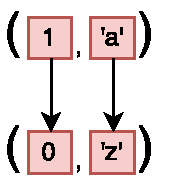
\includegraphics[scale=0.7]{images/parEval2}
\end{center}
We have only talked about the paralellization arrows of the same type up until now. But sometimes we want to paralellize heterogenous types as well. For this, we introduce a helper combinator \code{arrMaybe} first, that converts an arrow \code{arr a b} to an arrow \code{arr (Maybe a) (Maybe b)}.
\begin{lstlisting}[frame=htrbl]
arrMaybe :: (ArrowApply arr) => (arr a b) -> arr (Maybe a) (Maybe b)
arrMaybe fn = (arr $ go) >>> app
	where 
		go Nothing = (arr $ \Nothing -> Nothing, Nothing)
		go (Just a) = ((arr $ \(Just x) -> (fn, x)) >>> app >>> arr Just, (Just a))
\end{lstlisting}
With this, we can now easily write \code{parEval2} which combines two arrows \code{arr a b} and \code{arr c d} into a new parallel arrow \code{arr (a, c) (b, d)}. We start by converting both arrows with \code{arrMaybe}, combining them with \code{***} into a new arrow \code{arr (Maybe a, Maybe c) (Maybe b, Maybe d)}. This is then replicated twice and fed into parEvalN to get a \code{arr [(Maybe a, Maybe c)] [(Maybe b, Maybe d)]}. We can then apply this arrow to the input \code{[(Just a, Nothing), (Nothing, Just c)]} and then extract the resulting values with \code{fromJust} and the \code{!!} operator on lists in the last step.
\begin{lstlisting}[frame=htrbl]
parEval2 :: (ArrowParallel arr a b conf,
	ArrowParallel arr (Maybe a, Maybe c) (Maybe b, Maybe d) conf,
	ArrowApply arr) =>
	conf -> arr a b -> arr c d -> (arr (a, c) (b, d))
parEval2 conf f g =
	(arr $ \(a, c) -> (f_g, [(Just a, Nothing), (Nothing, Just c)])) >>>
	app >>>
	(arr $ \comb -> (fromJust (fst (comb !! 0)), fromJust (snd (comb !! 1))))
where
	f_g = parEvalN conf $ replicate 2 $ arrMaybe f *** arrMaybe g
\end{lstlisting}